\section{Analysis of the emerged languages}
\label{sec:analysis_language}
The languages that emerge are analyzed in two ways.
First, for each language that emerges through successful communication, a score is calculated that represents the similarity of the messages to valid English referring expressions.
In a second step, several languages are analyzed qualitatively, to determine what certain symbols mean and what they might refer to in the visual scenes.
\cmtDK[inline]{talks about why and which few languages}

To compare the emerged language to English in a \textbf{quantitative} way, a probing approach is used.
Probing can be used to analyze and interpret the hidden representations in neural networks.
Hereby, a second neural model is trained to predict selected linguistic properties on the basis of the hidden representations.
If this model is successfully able to predict the linguistic properties, the hidden representations are connected to them.
If second model can't be trained, it indicates that there is no correlation between the hidden representation and the linguistic property.
In the case of the emerged language, a neural model is trained to translate the messages of the sender into English referring expressions, based on the GRE algorithm by \citet{Dale1995}.
Recall, that this incremental is based on an order in salience for the attributes.
In English, \citet{Dale1995} propose the order of \emph{shape} > \emph{color} > \emph{size}.
However, there is no policy for the agents, that enforces specifically this order or indeed any salience order.
For this reason, the emerged languages are compared to all possible salience orders, given the three attributes \emph{shape}, \emph{color} and \emph{size}.
This will show if first, the languages follow any salience order and secondly, which attributes are more important for the agents to communicate.
% SD: The probing test is to show how well the emerged language can be trasnlated into English descriptions consistting of labels of scene features using Dale and Reiter idea of incrementality. However, we would need to know now what was the policy of the sender to generate message. Was this similar to Dale and Reiter to enforce longer descriptions?
% DK: done

The probing model consists of an encoder LSTM, one linear layer and a decoder LSTM.
The encoder LSTM encodes the messages of the emerged language.
Its final hidden state is used as a representation of the meaning of the complete message and passed through the linear layer, which learns an abstract representation of the message.
The dimension of the linear layer is kept small to prevent memorizing the dataset and force the model to find abstract connections between the input and the target.
The resulting vector is used as the initial state of the decoder LSTM.
The decoder LSTM is then trained to produce the English referring expression.
Both LSTMs have an embedding dimension of $LSTM_e=10$ and a hidden size of $LSTM_{out}=10$, while the linear layer has a size of $l=10$.
During decoding, teacher forcing is applied.
The success of the model is validated calculating cross entropy between the models predictions and the target English referring expression.
Since generalization doesn't play a role for probing, no dropout is applied and the model is trained and validated on the complete dataset; no test or validation split is used.
The models are trained for 200 epochs with a learning rate of $lr=0,004$ and a batch size of 32 samples per batch.

The translation model will learn two characteristics with this setup.
First, it can learn to find correlations between the emerged language and the English referring expressions, which is the goal of the probing.
But secondly, it can also learn underlying patterns in the English referring expressions that are independent of the emerged language.
For instance, it can learn that the referring expressions are likely to be two symbols long, or that for instance 'cube' is the most common shape.
This second characteristic will lead to a low loss during training, even though there are no connections to the emerged language.
In this test, only the first characteristic is interesting and would show the correlation between the emerged language and English referring expressions.
For that reason, two reference baselines are calculated for each salience order of the attributes, to eliminate the influence of the second characteristic.
% SD: Baselines?
% DK: (done)
The first baseline $L_{baseline}$ uses a non-informative input for the encoder LSTM, more specifically it always receives a vector of zeros and therefore can't learn any meaningful representation in the linear layer; the input for the decoder LSTM is the same for every sample.
By this, the model is trained to learn the structural patterns in the English referring expressions.
The resulting loss is the highest possible loss the model can achieve, independent of the input.
Resulting, if the emergent language is connected to English, the loss will be lower than this baseline.
If not, the loss will be as high as this baseline.
On the other side, the lowest possible loss $L_{English}$ is calculated, by using the English referring expressions as both input and target.
This verifies that the model is able to learn an abstract representation from the input and the resulting loss should be close to zero (since the input is perfectly correlated to the target).
These two references are used, to normalize the results of the actual emergent languages $L_{em}$, using the formula $L_{norm} = \frac{L_{em}-L_{English}}{L_{baseline} - L_{English}}$.
A loss close to $L_{baseline}$ will lead to 100\%, while a loss as $L_{English}$ will lead to 0\%.
% SD: Is this encessary? But when and where is this loss using 0 inouts calculated?
% DK: TODO, QUESTION
By doing this, all configurations can be compared directly to each other.
The lower $L_{norm}$, the higher the correlation between the emerged language and English referring expressions.

Tables \ref{tab:probing:discriminator:dale-2} to \ref{tab:probing:attention-predictor:colour} show the normalized losses $L_{norm}$ of the probing for the different tasks on all three datasets.
Hereby, only languages are listed for experiments in which the agents communicated successfully, that is $L_{norm}$ is lower than 100\%.
The first thing that can be noticed is that across almost all languages emerged through successful communication, $L_{norm}$ is lower than 100\% with at least one salience order, which shows that they make use of the attributes in some way.
On the other side, no language reaches an $L_{norm}$ close to 0, that is no language correlates perfectly with English referring expressions.
The closest is a language with $L_{norm}$ just above 40\%.
This shows that while many emerged languages have similarities with English, they make use of either other additional visual characteristics in the scenes or use different linguistic structures.

In the following paragraphs, languages will be referred to by their message length $n$ and their vocabulary size $|V|$ as $Lang_{n,|V|}$.

\begin{table}[ht]
    \centering
    \begin{tabular}{cc|c|c|c|c|c|c}
        \toprule
        $n$ & $|V|$ & \textbf{C > Sh > Si}              & \textbf{C > Si > Sh}              & \textbf{Sh > C > Si}     & \textbf{Sh > Si > C}     & \textbf{Si > C > Sh}     & \textbf{Si > Sh > C}     \\\midrule
        {1} & {2}   & \textcolor{red}{95,5\%}           & \textcolor{red}{97,57\%}          & {86,98\%}                & {81,43\%}                & \textcolor{red}{91,67\%} & {86,45\%}                \\
        {1} & {10}  & \textcolor{red}{96,11\%}          & \textcolor{red}{96,9\%}           & {89,61\%}                & {85\%}                   & {89,4\%}                 & {84,49\%}                \\
        {1} & {16}  & \textcolor{red}{95,19\%}          & \textcolor{red}{96,56\%}          & {87,25\%}                & {81,22\%}                & {89,34\%}                & {83,13\%}                \\
        {1} & {50}  & \textcolor{red}{96,61\%}          & \textcolor{red}{97,07\%}          & \textcolor{red}{91,26\%} & {85,75\%}                & {87,14\%}                & {82,61\%}                \\
        {1} & {100} & \textcolor{red}{95,91\%}          & \textcolor{red}{96,73\%}          & \textcolor{red}{90,63\%} & {86,01\%}                & {88,95\%}                & {84,17\%}                \\
        {2} & {2}   & \textcolor{red}{99,67\%}          & \textcolor{red}{99,91\%}          & \textcolor{red}{97,02\%} & \textcolor{red}{95,37\%} & \textcolor{red}{96,97\%} & \textcolor{red}{94,64\%} \\
        {2} & {10}  & \textcolor{red}{96,36\%}          & \textcolor{red}{96,34\%}          & \textcolor{red}{91,32\%} & {86,75\%}                & {87,69\%}                & {82,87\%}                \\
        {2} & {16}  & \textcolor{red}{95,63\%}          & \textcolor{red}{97,12\%}          & {88,11\%}                & {83,21\%}                & {89,86\%}                & {85,35\%}                \\
        {2} & {50}  & \textcolor{red}{95,34\%}          & \textcolor{red}{97,3\%}           & {85,48\%}                & {80,89\%}                & \textcolor{red}{92,22\%} & {86,18\%}                \\
        {2} & {100} & \textcolor{red}{94,88\%}          & \textcolor{red}{96,32\%}          & {87,37\%}                & {81,17\%}                & {88,35\%}                & {82,61\%}                \\
        {3} & {2}   & \textcolor{red}{\textbf{94,03\%}} & \textcolor{red}{96,96\%}          & \textbf{79,59\%}         & \textbf{74,54\%}         & \textcolor{red}{92,32\%} & {85,63\%}                \\
        {3} & {10}  & \textcolor{red}{96,1\%}           & \textcolor{red}{95,97\%}          & \textcolor{red}{90,45\%} & {84,84\%}                & {85,98\%}                & {80,5\%}                 \\
        {3} & {16}  & \textcolor{red}{95,71\%}          & \textcolor{red}{\textbf{95,1\%}}  & \textcolor{red}{90,97\%} & {85,33\%}                & {81\%}                   & \textbf{75,56\%}         \\
        {3} & {50}  & \textcolor{red}{96,32\%}          & \textcolor{red}{\textbf{94,55\%}} & \textcolor{red}{92,5\%}  & {86,81\%}                & \textbf{80,48\%}         & {75,73\%}                \\
        {3} & {100} & \textcolor{red}{95,33\%}          & \textcolor{red}{97,82\%}          & {86,05\%}                & {81,33\%}                & \textcolor{red}{93,91\%} & {88,54\%}                \\
        {4} & {2}   & \textcolor{red}{96,81\%}          & \textcolor{red}{95,12\%}          & \textcolor{red}{93,03\%} & {87,41\%}                & \textbf{80,73\%}         & \textbf{75,47\%}         \\
        {4} & {10}  & \textcolor{red}{95,31\%}          & \textcolor{red}{97,26\%}          & {86,9\%}                 & {82,67\%}                & \textcolor{red}{92,39\%} & {86,98\%}                \\
        {4} & {16}  & \textcolor{red}{95,63\%}          & \textcolor{red}{\textbf{94,65\%}} & \textcolor{red}{91,99\%} & {86,65\%}                & \textbf{79,23\%}         & \textbf{74,54\%}         \\
        {4} & {50}  & \textcolor{red}{94,76\%}          & \textcolor{red}{96,69\%}          & {86,8\%}                 & {81,33\%}                & {89,65\%}                & {83,92\%}                \\
        {4} & {100} & \textcolor{red}{96,16\%}          & \textcolor{red}{97,94\%}          & {89,57\%}                & {85,18\%}                & \textcolor{red}{92,56\%} & {87,74\%}                \\
        {6} & {2}   & \textcolor{red}{95,73\%}          & \textcolor{red}{96,99\%}          & {87,77\%}                & {83,27\%}                & \textcolor{red}{91,77\%} & {86,34\%}                \\
        {6} & {10}  & \textcolor{red}{\textbf{94,59\%}} & \textcolor{red}{99,89\%}          & {86,24\%}                & {81,46\%}                & \textcolor{red}{91,42\%} & {86,43\%}                \\
        {6} & {16}  & \textcolor{red}{95,51\%}          & \textcolor{red}{96,3\%}           & {88,89\%}                & {83,24\%}                & {87,61\%}                & {82,71\%}                \\
        {6} & {50}  & \textcolor{red}{\textbf{94,66\%}} & \textcolor{red}{97,43\%}          & \textbf{84,93\%}         & \textbf{78,61\%}         & \textcolor{red}{91,48\%} & {83,66\%}                \\
        {6} & {100} & \textcolor{red}{95,37\%}          & \textcolor{red}{97,77\%}          & \textbf{83,75\%}         & \textbf{80,84\%}         & \textcolor{red}{93,96\%} & {89,02\%}                \\
        \bottomrule
    \end{tabular}
    \caption{Normalized losses $L_{norm}$ of the probing model on emerged languages of the \emph{discrimination games} on the 'Dale-2' dataset. The emerged languages are probed with different salience orders where 'C' corresponds to the \emph{color}, 'Sh' to the \emph{shape} and 'Si' to the \emph{size}. The table only includes languages, with which the agents could successfully solve the task.}
    \label{tab:probing:discriminator:dale-2}
\end{table}

Looking at the results for the discriminator, one can see that the results are very different for each dataset.
On the 'Dale-2' dataset $L_{norm}$ is relatively high for all salience orders (see Table \ref{tab:probing:discriminator:dale-2}).
Yet, the correlation to English referring expressions with the \emph{color} as most important attribute is the lowest.
When the \emph{color} attribute is in the second position, the correlation becomes higher, but the highest correlation is achieved when the \emph{color} has the least importance.
This shows that the agents don't use the \emph{color} in the communication, but rather rely on \emph{shape} and \emph{size}.
The order of importance of these attributes however is not as clear.
For some combinations of the message length $n$ and vocabulary size $|V|$, the \emph{size} seems to be the dominant attribute, while for others the \emph{shape} seems more important in the communication.
Interestingly, one can see that for many languages only one salience order has a low $L_{norm}$, while the $L_{norm}$ for the remaining salience orders with a different attribute in the first position is higher.
This applies for example to $Lang_{3,2}$, where the loss for 'Sh > Si > C' is 74,54\% while the second lowest is only at 85,63\% for 'Si > Sh > C'.
The same can be seen for instance for $Lang_{3,16}$ in the other direction.
This difference indicates that the agents are relying mostly on the most important attribute of this salience order to discriminate the target object.
If the $L_{norm}$ for instance were similar for the salience orders 'Sh > Si > C' and 'Si > Sh > C', this would mean that the emerged language could be connected to both salience orders in the same way.
Following, the agents would use the \emph{shape} as often as \emph{size} to discriminate the objects.
This is however only the case on the 'Dale-2' dataset when the loss is higher (for instance languages $Lang_{2,16}$, $Lang_{2,100}$ or $Lang_{6,16}$).
Since the lowest $L_{norm}$ with 74,54\% is still very high compared to a complete correlation (0\%), the agents seem to encode additionally other information in their messages.

Looking at the influence of $n$ and $|V|$, one can see that across almost all values, there is at least some correlation to one salience order.
The correlation seems to be highest with $n \in \{3,4\}$, where the loss can reach down 74,54\%.
Hereby, the most important attribute in the messages seems to be the \emph{size}.
For the remaining message lengths $n$, the loss stays mostly between 80\% and 85\%.
For $n \in \{2,6\}$ the \emph{shape} seems to be the most dominant attribute, while for $n=1$ the \emph{size} and \emph{shape} seem to have a similar importance.
The influence of the vocabulary size $|V|$ is not as clear.
Small to medium-sized vocabularies seem to promote higher correlations with English referring expressions, but also languages with $|V|=100$ can reach losses of around 80\%.

\begin{table}[ht]
    \centering
    \begin{tabular}{cc|c|c|c|c|c|c}
        \toprule
        $n$ & $|V|$ & \textbf{C > Sh > Si}     & \textbf{C > Si > Sh}     & \textbf{Sh > C > Si}     & \textbf{Sh > Si > C}     & \textbf{Si > C > Sh} & \textbf{Si > Sh > C} \\\midrule
        {1} & {2}   & \textcolor{red}{94,96\%} & \textcolor{red}{91,27\%} & \textcolor{red}{94,51\%} & \textcolor{red}{90,99\%} & {88,52\%}            & {88,17\%}            \\
        {1} & {10}  & {84,34\%}                & {84,03\%}                & {80,91\%}                & {73,23\%}                & {79,95\%}            & {72,34\%}            \\
        {1} & {16}  & {86,27\%}                & {84,96\%}                & {82,76\%}                & {75,35\%}                & {80,72\%}            & {74,04\%}            \\
        {1} & {50}  & {85,95\%}                & {84,4\%}                 & {82,96\%}                & {74,97\%}                & {80,2\%}             & {73,54\%}            \\
        {1} & {100} & {86,31\%}                & {85,58\%}                & {82,9\%}                 & {76,03\%}                & {81,64\%}            & {74,62\%}            \\
        {2} & {10}  & \textbf{82,66\%}         & {83,23\%}                & \textbf{78,51\%}         & {71,01\%}                & {78,89\%}            & {70,61\%}            \\
        {2} & {16}  & {89,78\%}                & {85,53\%}                & {87,68\%}                & {80,64\%}                & {81,06\%}            & {77,24\%}            \\
        {2} & {50}  & {84,4\%}                 & {82,65\%}                & {80,62\%}                & {71,42\%}                & {77,53\%}            & {69,46\%}            \\
        {2} & {100} & {89,65\%}                & {85,3\%}                 & {87,26\%}                & {79,91\%}                & {80,88\%}            & {77,1\%}             \\
        {3} & {2}   & {87,19\%}                & {86,93\%}                & {83,99\%}                & {78,18\%}                & {83,65\%}            & {77,08\%}            \\
        {3} & {10}  & {87,15\%}                & {84,67\%}                & {84,01\%}                & {76,24\%}                & {80,41\%}            & {74,11\%}            \\
        {3} & {50}  & \textbf{82,98\%}         & {82,25\%}                & {78,85\%}                & {70,62\%}                & {77,42\%}            & {69,27\%}            \\
        {3} & {100} & {83,78\%}                & {83,07\%}                & {80,23\%}                & {72,15\%}                & {78,94\%}            & {71,1\%}             \\
        {4} & {2}   & {89,23\%}                & {87,43\%}                & {87,09\%}                & {81,45\%}                & {83,83\%}            & {79,11\%}            \\
        {4} & {10}  & {88,66\%}                & {84,83\%}                & {85,9\%}                 & {78,98\%}                & {80,2\%}             & {75,64\%}            \\
        {4} & {16}  & {83,14\%}                & \textbf{81,51\%}         & \textbf{78,15\%}         & \textbf{70,21\%}         & \textbf{77,32\%}     & \textbf{68,48\%}     \\
        {4} & {50}  & {87,62\%}                & {84,38\%}                & {85,25\%}                & {77,29\%}                & {79,94\%}            & {74,03\%}            \\
        {4} & {100} & \textcolor{red}{90,17\%} & {85,76\%}                & {87,68\%}                & {80,71\%}                & {81,37\%}            & {78,1\%}             \\
        {6} & {10}  & \textbf{82,03\%}         & \textbf{80,51\%}         & \textbf{77,46\%}         & \textbf{68,63\%}         & \textbf{75,71\%}     & \textbf{67,15\%}     \\
        {6} & {16}  & {84,73\%}                & \textbf{81,12\%}         & {80,99\%}                & \textbf{70,5\%}          & \textbf{76,06\%}     & \textbf{69,12\%}     \\
        {6} & {50}  & {86,95\%}                & {85,13\%}                & {84,06\%}                & {76,95\%}                & {80,11\%}            & {74,51\%}            \\
        {6} & {100} & {86,15\%}                & {82,19\%}                & {83,56\%}                & {75,56\%}                & {77,76\%}            & {72,47\%}            \\
        \bottomrule
    \end{tabular}
    \caption{Normalized losses $L_{norm}$ of the probing model on emerged languages of the \emph{discrimination games} on the 'Dale-5' dataset. The emerged languages are probed with different salience orders where 'C' corresponds to the \emph{color}, 'Sh' to the \emph{shape} and 'Si' to the \emph{size}. The table only includes languages, with which the agents could successfully solve the task.}
    \label{tab:probing:discriminator:dale-5}
\end{table}

The emerged languages on the 'Dale-5' dataset have generally a higher correlation to English referring expressions (see Table \ref{tab:probing:discriminator:dale-5}).
For almost all salience orders and emerged languages, the loss is lower than 90\%.
In the best cases, it even reaches down to 67,15\%.
Again, the \emph{size} and the \emph{shape} are mostly communicated between the agents, but the \emph{color} now plays a bigger role in the messages.
The agents seem to need to rely on more attributes to discriminate the target object.
This aligns also with English referring expressions, where the average length of the referring expressions across the whole 'Dale-5' dataset is longer than for the 'Dale-2' dataset.
However, opposed to the 'Dale-2' dataset, there are almost no languages, where there is one dominant attribute.
More often the loss is similar for two salience orders with different primary attributes.
For instance the salience orders 'Sh > Si > C' and 'Si > Sh > C' both provide losses around 70\% for $Lang_{6,16}$.
Only the languages $Lang_{2,16}$, $Lang_{4,10}$, $Lang_{4,50}$ and $Lang_{6,100}$ have differences of more than 3\% points for these salience orders.
This indicates, that the agents make use of both \emph{shape} and \emph{size} similarly often, while the \emph{color} is used for much fewer images.

When the agents are able to produce longer messages, their languages seem to have more similarities with possible English languages.
With $n>1$ the agents produce languages that can have losses lower than 70\% for the salience order 'Si > Sh > C'.
Yet, languages with $n=1$ are not far off and have mostly losses between 72\% and 75\%.
Looking at the vocabulary size, languages with $|V|=2$ are less likely to emerge and if they emerge they have a lower correlation with English.
The best results are produces with $|V| \in \{10,16\}$ for longer messages (for instance $Lang_{4,16}$, $Lang_{6,10}$ and $Lang_{6,16}$), while shorter messages fare generally better with a larger vocabulary of $|V| \in \{50,100\}$ ($Lang_{2,50}$, $Lang_{3,50}$ and $Lang_{3,100}$).

\begin{table}[ht]
    \centering
    \begin{tabular}{cc|c|c|c|c|c|c}
        \toprule
        $n$ & $|V|$ & \textbf{C > Sh > Si}     & \textbf{C > Si > Sh}     & \textbf{Sh > C > Si}     & \textbf{Sh > Si > C}     & \textbf{Si > C > Sh}     & \textbf{Si > Sh > C}     \\\midrule
        {1} & {2}   & \textcolor{red}{91,62\%} & \textcolor{red}{91,57\%} & \textcolor{red}{94,31\%} & \textcolor{red}{95,13\%} & \textcolor{red}{93,11\%} & \textcolor{red}{94,92\%} \\
        {1} & {10}  & {79,08\%}                & {79,08\%}                & {85,04\%}                & {86,86\%}                & {82,37\%}                & {86,38\%}                \\
        {1} & {16}  & {84,02\%}                & {83,96\%}                & {88,67\%}                & {89,65\%}                & {86,36\%}                & {89,36\%}                \\
        {1} & {50}  & \textcolor{red}{93,88\%} & \textcolor{red}{93,74\%} & \textcolor{red}{95,03\%} & \textcolor{red}{95,49\%} & \textcolor{red}{94,64\%} & \textcolor{red}{95,35\%} \\
        {2} & {10}  & {88,67\%}                & {88,36\%}                & {89,59\%}                & \textcolor{red}{90,77\%} & \textcolor{red}{90,01\%} & {89,81\%}                \\
        {2} & {16}  & {81,13\%}                & {81,02\%}                & {86,16\%}                & {87,97\%}                & {83,85\%}                & {87,56\%}                \\
        {3} & {2}   & {83,38\%}                & {83,46\%}                & {88,21\%}                & {89,71\%}                & {86,05\%}                & {89,37\%}                \\
        {3} & {10}  & \textbf{77\%}            & \textbf{76,77\%}         & \textbf{83,54\%}         & \textbf{85,57\%}         & \textbf{79,97\%}         & \textbf{84,9\%}          \\
        {3} & {16}  & \textcolor{red}{93,52\%} & \textcolor{red}{93,6\%}  & \textcolor{red}{94,16\%} & \textcolor{red}{94,14\%} & \textcolor{red}{93,75\%} & \textcolor{red}{93,55\%} \\
        {4} & {10}  & \textbf{68,04\%}         & \textbf{66,51\%}         & \textbf{76,33\%}         & \textbf{78,56\%}         & \textbf{71,42\%}         & \textbf{78,56\%}         \\
        {4} & {16}  & \textbf{75,1\%}          & \textbf{74,93\%}         & \textbf{81,2\%}          & \textbf{83,35\%}         & \textbf{77,6\%}          & \textbf{82,76\%}         \\
        {6} & {2}   & {84,21\%}                & {84,02\%}                & {88,41\%}                & {89,77\%}                & {86,61\%}                & {89,35\%}                \\
        \bottomrule
    \end{tabular}
    \caption{Normalized losses $L_{norm}$ of the probing model on emerged languages of the \emph{discrimination games} on the 'CLEVR color' dataset. The emerged languages are probed with different salience orders where 'C' corresponds to the \emph{color}, 'Sh' to the \emph{shape} and 'Si' to the \emph{size}. The table only includes languages, with which the agents could successfully solve the task.}
    \label{tab:probing:discriminator:colour}
\end{table}

Finally on the 'CLEVR color' dataset, much fewer languages emerge (see Table \ref{tab:probing:discriminator:colour}).
Those languages that emerge have very different levels of correlation to English
While three languages stay above 90\% for all salience orders, most of them stay between 80\% and 90\%.
Four languages even get below 80\% for the salience orders where the \emph{color} is the most important attribute.
One of those even reaches 66,51\%, the highest correlation across all emerged languages on the discrimination task.
Unsurprisingly, the \emph{color} is now the most important attribute.
The loss with the remaining salience orders is still relatively low, but this is likely due to the fact, that the color occurs in any referring expression as it is the only discriminating attribute.
The probing model can therefore easily connect this pattern to the emerged language.
As expected, the losses for 'Sh > Si > C' and 'Si > Sh > C' are almost the same, which indicates that the agents make (no) use of both \emph{shape} and \emph{size} in the same way.

Even though only one attribute would need to be communicated, languages with $n \in \{3,4\}$ tend to be closer to English referring expressions.
Hereby, vocabulary sizes of $|V| \in \{10,16\}$ produce the most correlating languages, while languages with only 2 symbols have relatively high losses.
The agents were not able to communicate with vocabulary sizes larger than 16.


\begin{table}[ht]
    \centering
    \begin{tabular}{cc|c|c|c|c|c|c}
        \toprule
        $n$ & $|V|$ & \textbf{C > Sh > Si}     & \textbf{C > Si > Sh}              & \textbf{Sh > C > Si}     & \textbf{Sh > Si > C}     & \textbf{Si > C > Sh}     & \textbf{Si > Sh > C}     \\\midrule
        {1} & {2}   & \textcolor{red}{95,07\%} & \textcolor{red}{98,06\%}          & {86,63\%}                & {85,3\%}                 & \textcolor{red}{96,26\%} & \textcolor{red}{93,32\%} \\
        {1} & {10}  & \textcolor{red}{90,8\%}  & \textcolor{red}{96,4\%}           & {71,88\%}                & {69,29\%}                & \textcolor{red}{94,05\%} & {85,13\%}                \\
        {1} & {16}  & \textcolor{red}{91,47\%} & \textcolor{red}{96,96\%}          & {71,2\%}                 & {66,82\%}                & \textcolor{red}{93,83\%} & {83,35\%}                \\
        {1} & {50}  & \textcolor{red}{93,26\%} & \textcolor{red}{96,63\%}          & {77,53\%}                & {71,94\%}                & \textcolor{red}{93,56\%} & {84,62\%}                \\
        {1} & {100} & \textcolor{red}{93,5\%}  & \textcolor{red}{97,86\%}          & {77,42\%}                & {71,93\%}                & \textcolor{red}{94,68\%} & {85,77\%}                \\
        {2} & {2}   & \textcolor{red}{93,57\%} & \textcolor{red}{97,72\%}          & {80,89\%}                & {79,8\%}                 & \textcolor{red}{96,08\%} & \textcolor{red}{90,71\%} \\
        {2} & {10}  & \textbf{84,86\%}         & \textcolor{red}{\textbf{92,07\%}} & {58,8\%}                 & \textbf{52,09\%}         & \textbf{88,36\%}         & {77,01\%}                \\
        {2} & {16}  & {87,29\%}                & \textcolor{red}{92,88\%}          & {68,52\%}                & {71,5\%}                 & \textcolor{red}{92,56\%} & {83,9\%}                 \\
        {2} & {50}  & {89,15\%}                & \textcolor{red}{95\%}             & {68,19\%}                & {68,93\%}                & \textcolor{red}{93,11\%} & {83,95\%}                \\
        {2} & {100} & \textcolor{red}{91,06\%} & \textcolor{red}{96,14\%}          & {71,98\%}                & {67,23\%}                & \textcolor{red}{92,81\%} & {82,71\%}                \\
        {3} & {2}   & \textcolor{red}{93,05\%} & \textcolor{red}{97,15\%}          & {82,41\%}                & {77,36\%}                & \textcolor{red}{94,43\%} & {88,8\%}                 \\
        {3} & {10}  & {88,52\%}                & \textcolor{red}{95,41\%}          & {66,61\%}                & {63,63\%}                & \textcolor{red}{92,25\%} & {81,46\%}                \\
        {3} & {16}  & {85,71\%}                & \textcolor{red}{92,88\%}          & \textbf{56,44\%}         & \textbf{49,22\%}         & \textbf{88,87\%}         & \textbf{74,54\%}         \\
        {3} & {50}  & \textcolor{red}{90,78\%} & \textcolor{red}{96,28\%}          & {68,17\%}                & {64,84\%}                & \textcolor{red}{94,16\%} & {83,5\%}                 \\
        {3} & {100} & {86,54\%}                & \textcolor{red}{93,54\%}          & {65,9\%}                 & {66,03\%}                & \textcolor{red}{92,49\%} & {83,28\%}                \\
        {4} & {10}  & {87,61\%}                & \textcolor{red}{94,63\%}          & {66,83\%}                & {64,85\%}                & \textcolor{red}{92,24\%} & {82,85\%}                \\
        {4} & {16}  & \textbf{85,7\%}          & \textcolor{red}{93,56\%}          & \textbf{56,9\%}          & \textbf{52,1\%}          & \textbf{88,98\%}         & \textbf{76,15\%}         \\
        {4} & {50}  & {87,55\%}                & \textcolor{red}{94,24\%}          & {61,03\%}                & {55,82\%}                & \textcolor{red}{91,73\%} & \textbf{76,52\%}         \\
        {4} & {100} & {88,84\%}                & \textcolor{red}{94,84\%}          & {68,68\%}                & {66,73\%}                & \textcolor{red}{92,57\%} & {81,79\%}                \\
        {6} & {2}   & \textcolor{red}{93,48\%} & \textcolor{red}{98,14\%}          & {81,36\%}                & {79,08\%}                & \textcolor{red}{96,09\%} & \textcolor{red}{90,95\%} \\
        {6} & {10}  & \textbf{85\%}            & \textcolor{red}{\textbf{92,44\%}} & \textbf{57,21\%}         & {55,07\%}                & {89,39\%}                & {77,44\%}                \\
        {6} & {16}  & {88,02\%}                & \textcolor{red}{94,22\%}          & {71,42\%}                & {66,35\%}                & \textcolor{red}{90,86\%} & {84,12\%}                \\
        {6} & {50}  & \textcolor{red}{98,57\%} & \textcolor{red}{99,45\%}          & \textcolor{red}{95,57\%} & \textcolor{red}{95,06\%} & \textcolor{red}{99,16\%} & \textcolor{red}{96,64\%} \\
        {6} & {100} & {86,44\%}                & \textcolor{red}{\textbf{92,76\%}} & {65,59\%}                & {65,93\%}                & \textcolor{red}{92,42\%} & {82,16\%}                \\
        \bottomrule
    \end{tabular}
    \caption{Normalized losses $L_{norm}$ of the probing model on emerged languages of the \emph{referring expression generation games} on the 'Dale-2' dataset. The emerged languages are probed with different salience orders where 'C' corresponds to the \emph{color}, 'Sh' to the \emph{shape} and 'Si' to the \emph{size}. The table only includes languages, with which the agents could successfully solve the task.}
    \label{tab:probing:re-generator:dale-2}
\end{table}

Tables \ref{tab:probing:re-generator:dale-2} and \ref{tab:probing:re-generator:dale-5} show the results of the probing on the emerged languages of the \emph{referring expression generation games}.
This is the only task, where the final task for the agents is to generate English referring expressions with the salience order 'Sh > C > Si'.
English referring expressions are therefore explicitly passed to the agents as correct labels during training.
One can therefore expect the agents to align their own language with the target referring expressions and a high correlation with the salience order 'Sh > C > Si' is expected.
Looking at the results, this is partially confirmed for the 'Dale-2' dataset.
Some emerged languages reach with a normalized loss of 49,22\% one of the highest correlations to English referring expressions across all emerged languages in this thesis.
However, the salience order with the highest correlation is 'Sh > Si > C', and values the \emph{size} more than the \emph{color}, instead of the reversed way as in the training data of the agents.
The color seems, as in the previous task, not as important to communicate as the other attributes.
While the \emph{size} plays a bigger role, the \emph{shape} is the central attribute in the communication.
This fact is interesting for two reasons:
First, the \emph{shape} being the most important attribute in the messages aligns with the receiver's generated referring expressions where the \emph{shape} was predicted almost perfectly.
The receiver therefore seems to make use of the sender's ability to extract the \emph{shape} from the images and reproduces what the sender communicated.
However, without a deeper analysis, it can't be ruled out that the receiver extracts the \emph{shape} themselves from the image, and uses the sender's message only to determine the correct target object in the scene.
Secondly, this does not apply to the \emph{size} and the \emph{color}.
While the size seems to be communicated, it is not generated correctly by the receiver.
The opposite applies to the \emph{color}.
The \emph{color} is not important in the communication, but the receiver however is able to produce correct colors in the generated referring expression.
This shows that the agents actually don't align their own language with the target referring expression.
The communication of the target object between the agents seems to be a separate step from the receiver's generation of the referring expression.

Looking at the influence of the message length, one can see that the language is the least correlated to the salience order 'Sh > Si > C' with $n=1$.
Still, even with these short messages, the loss can go down to 66,82\%.
With $n>1$, almost all languages have a loss of below 70\%, while at least one configuration is even lower than 60\%.
Hereby, languages with $n \in \{3,4\}$ have the highest correlation to English.
Languages with the highest correlation also mostly make use of a medium-sized vocabulary of $|V| \in \{10,16\}$ as for example $Lang_{2,10}$, $Lang_{3,16}$, $Lang_{4,16}$ and $Lang_{6,10}$.
While larger vocabularies, can still correlate relatively much with English referring expressions, languages with $|V|=2$ are much less similar.

\begin{table}[ht]
    \centering
    \begin{tabular}{cc|c|c|c|c|c|c}
        \toprule
        $n$ & $|V|$ & \textbf{C > Sh > Si}     & \textbf{C > Si > Sh}     & \textbf{Sh > C > Si}     & \textbf{Sh > Si > C} & \textbf{Si > C > Sh}     & \textbf{Si > Sh > C}     \\\midrule
        {1} & {2}   & \textcolor{red}{92,86\%} & \textcolor{red}{96,4\%}  & \textcolor{red}{90,06\%} & {89,5\%}             & \textcolor{red}{95,73\%} & \textcolor{red}{90,93\%} \\
        {1} & {10}  & {83,9\%}                 & \textcolor{red}{90,9\%}  & {78,63\%}                & {74,74\%}            & {89,6\%}                 & {78,99\%}                \\
        {1} & {16}  & {84,68\%}                & \textcolor{red}{91,65\%} & {80,11\%}                & {77,03\%}            & \textcolor{red}{90,16\%} & {81,05\%}                \\
        {1} & {50}  & {84,85\%}                & \textcolor{red}{91,67\%} & {79,95\%}                & {77,11\%}            & \textcolor{red}{90,32\%} & {81,04\%}                \\
        {2} & {2}   & \textcolor{red}{90,51\%} & \textcolor{red}{95,36\%} & {87,5\%}                 & {86,43\%}            & \textcolor{red}{94,77\%} & {88,35\%}                \\
        {2} & {10}  & {82,44\%}                & \textcolor{red}{90,32\%} & {77,65\%}                & {73,73\%}            & {88,89\%}                & {78,41\%}                \\
        {2} & {16}  & {81,85\%}                & \textbf{89,4\%}          & {76,07\%}                & \textbf{71,66\%}     & {87,9\%}                 & \textbf{75,91\%}         \\
        {2} & {50}  & {83,58\%}                & \textcolor{red}{91,12\%} & {78,67\%}                & {75,03\%}            & {89,94\%}                & {79,06\%}                \\
        {3} & {2}   & \textcolor{red}{92,51\%} & \textcolor{red}{95,96\%} & {89,96\%}                & {88,7\%}             & \textcolor{red}{95,18\%} & \textcolor{red}{90,43\%} \\
        {3} & {10}  & {82,11\%}                & {89,54\%}                & {75,9\%}                 & {71,78\%}            & {88,18\%}                & {76,72\%}                \\
        {3} & {50}  & {83,12\%}                & \textcolor{red}{90,82\%} & {77,62\%}                & {74,08\%}            & {88,88\%}                & {78,74\%}                \\
        {3} & {100} & {83,74\%}                & {89,59\%}                & {79,29\%}                & {74,48\%}            & \textbf{87,46\%}         & {78,05\%}                \\
        {4} & {2}   & {88,86\%}                & \textcolor{red}{94\%}    & {84,8\%}                 & {83,19\%}            & \textcolor{red}{93,37\%} & {85,92\%}                \\
        {4} & {10}  & \textbf{79,93\%}         & \textbf{89,29\%}         & \textbf{74,1\%}          & \textbf{69,5\%}      & \textbf{87,19\%}         & \textbf{74,79\%}         \\
        {4} & {16}  & \textbf{81,26\%}         & {89,68\%}                & \textbf{75,73\%}         & {71,96\%}            & {88,4\%}                 & {76,93\%}                \\
        {4} & {50}  & {81,55\%}                & {89,42\%}                & {75,9\%}                 & {71,68\%}            & {88,17\%}                & {76,55\%}                \\
        {6} & {2}   & \textcolor{red}{91,09\%} & \textcolor{red}{95,26\%} & {87,86\%}                & {86,81\%}            & \textcolor{red}{94,78\%} & {88,82\%}                \\
        {6} & {50}  & \textbf{80,39\%}         & \textbf{87,85\%}         & \textbf{75,01\%}         & \textbf{68,71\%}     & \textbf{84,54\%}         & \textbf{72,93\%}         \\
        \bottomrule
    \end{tabular}
    \caption{Normalized losses $L_{norm}$ of the probing model on emerged languages of the \emph{referring expression generation games} on the 'Dale-5' dataset. The emerged languages are probed with different salience orders where 'C' corresponds to the \emph{color}, 'Sh' to the \emph{shape} and 'Si' to the \emph{size}. The table only includes languages, with which the agents could successfully solve the task.}
    \label{tab:probing:re-generator:dale-5}
\end{table}

On the 'Dale-5' dataset, the emerged languages again resemble the English referring expressions less.
While the dominant salience order is 'Sh > Si > C' as on the 'Dale-2' dataset, the \emph{color} plays a bigger role.
This effect is the same as for the discrimination games, and can be explained by the higher number or distractors.
While the loss for the salience order 'Sh > Si > C' is lower than 70\% for two languages, it stays between 70\% and 80\% for most.


\begin{table}[ht]
    \centering
    \begin{tabular}{cc|c|c|c|c|c|c}
        \toprule
        $n$ & $|V|$ & \textbf{C > Sh > Si}     & \textbf{C > Si > Sh}     & \textbf{Sh > C > Si}     & \textbf{Sh > Si > C}     & \textbf{Si > C > Sh}      & \textbf{Si > Sh > C}      \\\midrule
        {1} & {2}   & \textcolor{red}{95,73\%} & \textcolor{red}{94,23\%} & \textcolor{red}{92,96\%} & \textcolor{red}{90,59\%} & {81,59\%}                 & {78,21\%}                 \\
        {1} & {10}  & \textcolor{red}{91,77\%} & \textcolor{red}{91,19\%} & {73,14\%}                & {63,99\%}                & {67,45\%}                 & {57,55\%}                 \\
        {1} & {16}  & \textcolor{red}{91,74\%} & \textcolor{red}{90,87\%} & {73,07\%}                & {63,78\%}                & {66,16\%}                 & {55,48\%}                 \\
        {1} & {50}  & \textcolor{red}{97,78\%} & \textcolor{red}{93,1\%}  & \textcolor{red}{94,22\%} & {87,45\%}                & {69,23\%}                 & {64,97\%}                 \\
        {1} & {100} & \textcolor{red}{97,91\%} & \textcolor{red}{93,1\%}  & \textcolor{red}{94,18\%} & {87,35\%}                & {69,25\%}                 & {64,99\%}                 \\
        {2} & {2}   & \textcolor{red}{93,17\%} & \textcolor{red}{91,69\%} & {81,96\%}                & {75,97\%}                & {72,05\%}                 & {64,29\%}                 \\
        {2} & {10}  & \textcolor{red}{94,07\%} & \textcolor{red}{98,04\%} & {75,32\%}                & {71,91\%}                & \textcolor{red}{94,38\%}  & {86,62\%}                 \\
        {2} & {16}  & \textcolor{red}{97,72\%} & \textcolor{red}{92,9\%}  & \textcolor{red}{94,18\%} & {87,09\%}                & {68,54\%}                 & {64,13\%}                 \\
        {2} & {50}  & \textcolor{red}{97,87\%} & \textcolor{red}{93,08\%} & \textcolor{red}{94,25\%} & {87,54\%}                & {69,2\%}                  & {65,17\%}                 \\
        {2} & {100} & {89,6\%}                 & \textbf{89,58\%}         & \textbf{65,65\%}         & \textbf{55,69\%}         & {64,92\%}                 & {53,53\%}                 \\
        {3} & {2}   & \textcolor{red}{97,73\%} & \textcolor{red}{99,28\%} & \textcolor{red}{95,84\%} & \textcolor{red}{97,72\%} & \textcolor{red}{101,58\%} & \textcolor{red}{100,22\%} \\
        {3} & {10}  & \textcolor{red}{91,04\%} & \textcolor{red}{90,52\%} & {71,06\%}                & {61,36\%}                & {65,59\%}                 & {54,93\%}                 \\
        {3} & {16}  & \textcolor{red}{91,09\%} & \textcolor{red}{90,3\%}  & {71,71\%}                & {62,42\%}                & {66,28\%}                 & {56,16\%}                 \\
        {3} & {50}  & \textcolor{red}{97,07\%} & \textcolor{red}{91,72\%} & \textcolor{red}{92,7\%}  & {85,33\%}                & {66,38\%}                 & {61,26\%}                 \\
        {3} & {100} & \textcolor{red}{97,81\%} & \textcolor{red}{93,01\%} & \textcolor{red}{94,16\%} & {87,3\%}                 & {68,83\%}                 & {64,6\%}                  \\
        {4} & {2}   & \textcolor{red}{91,95\%} & \textcolor{red}{96,87\%} & {73,55\%}                & {72,66\%}                & \textcolor{red}{98,37\%}  & \textcolor{red}{90,23\%}  \\
        {4} & {10}  & \textcolor{red}{97,7\%}  & \textcolor{red}{93,1\%}  & \textcolor{red}{94,16\%} & {87,24\%}                & {69,22\%}                 & {64,81\%}                 \\
        {4} & {16}  & \textbf{86,75\%}         & \textbf{89\%}            & \textbf{57,02\%}         & \textbf{44,33\%}         & \textbf{63,78\%}          & \textbf{48,21\%}          \\
        {4} & {50}  & \textcolor{red}{90,86\%} & \textcolor{red}{90,5\%}  & {71,22\%}                & {61,09\%}                & {65,26\%}                 & {54,87\%}                 \\
        {4} & {100} & \textcolor{red}{96,4\%}  & \textcolor{red}{90,22\%} & \textcolor{red}{92,44\%} & {83,78\%}                & \textbf{59,98\%}          & {54,38\%}                 \\
        {6} & {2}   & \textcolor{red}{90,06\%} & \textcolor{red}{90,46\%} & {71,62\%}                & {64,56\%}                & {70,67\%}                 & {61,35\%}                 \\
        {6} & {10}  & \textbf{88,38\%}         & \textcolor{red}{90,24\%} & \textbf{63,68\%}         & \textbf{53,21\%}         & \textbf{64,22\%}          & \textbf{52,19\%}          \\
        {6} & {16}  & \textbf{89,01\%}         & \textbf{89,74\%}         & {67,03\%}                & {56,73\%}                & {64,44\%}                 & \textbf{52,78\%}          \\
        {6} & {50}  & \textcolor{red}{97,68\%} & \textcolor{red}{92,77\%} & \textcolor{red}{97,03\%} & {87,24\%}                & {68,51\%}                 & {64,27\%}                 \\
        {6} & {100} & {89,84\%}                & {89,81\%}                & {69,75\%}                & {60,55\%}                & {65,19\%}                 & {54,93\%}                 \\
        \bottomrule
    \end{tabular}
    \caption{Normalized losses $L_{norm}$ of the probing model on emerged languages of the \emph{attribute generation games} on the 'Dale-2' dataset. The emerged languages are probed with different salience orders where 'C' corresponds to the \emph{color}, 'Sh' to the \emph{shape} and 'Si' to the \emph{size}. The table only includes languages, with which the agents could successfully solve the task.}
    \label{tab:probing:attribute-generator:dale-2}
\end{table}

\begin{table}[ht]
    \centering
    \begin{tabular}{cc|c|c|c|c|c|c}
        \toprule
        $n$ & $|V|$ & \textbf{C > Sh > Si}     & \textbf{C > Si > Sh}     & \textbf{Sh > C > Si}     & \textbf{Sh > Si > C}     & \textbf{Si > C > Sh}     & \textbf{Si > Sh > C}     \\\midrule
        {1} & {2}   & \textcolor{red}{91,81\%} & \textcolor{red}{96,22\%} & {89,08\%}                & {88,2\%}                 & \textcolor{red}{95,91\%} & \textcolor{red}{90,3\%}  \\
        {1} & {10}  & {83,4\%}                 & {82,11\%}                & {79,68\%}                & {67,88\%}                & {77,12\%}                & {66,75\%}                \\
        {1} & {16}  & {86,76\%}                & {87,06\%}                & {83,08\%}                & {75,03\%}                & {83,79\%}                & {74,72\%}                \\
        {1} & {50}  & {83,12\%}                & {82\%}                   & {78,81\%}                & {66,76\%}                & {76,95\%}                & {65,95\%}                \\
        {1} & {100} & \textcolor{red}{93,84\%} & {87,09\%}                & \textcolor{red}{93,01\%} & {83,36\%}                & {82,19\%}                & {79,14\%}                \\
        {2} & {2}   & {88,86\%}                & {86,82\%}                & {86,62\%}                & {78,45\%}                & {82,59\%}                & {76,49\%}                \\
        {2} & {10}  & {83,91\%}                & {81,57\%}                & {79,76\%}                & {67,89\%}                & {76,47\%}                & {66,1\%}                 \\
        {2} & {16}  & \textbf{75,6\%}          & \textbf{77,74\%}         & \textbf{68,78\%}         & \textbf{55,43\%}         & \textbf{72,24\%}         & \textbf{56,24\%}         \\
        {2} & {50}  & {85,1\%}                 & {83,08\%}                & {81,27\%}                & {70,13\%}                & {77,86\%}                & {68,54\%}                \\
        {2} & {100} & {83,24\%}                & {81,87\%}                & {79,02\%}                & {67,32\%}                & {77,06\%}                & {66,19\%}                \\
        {3} & {2}   & \textcolor{red}{97,21\%} & \textcolor{red}{96,08\%} & \textcolor{red}{96,43\%} & \textcolor{red}{95,23\%} & \textcolor{red}{95,18\%} & \textcolor{red}{94,24\%} \\
        {3} & {10}  & {82,66\%}                & {81,11\%}                & {78,38\%}                & {66,21\%}                & {75,68\%}                & {64,52\%}                \\
        {3} & {16}  & \textcolor{red}{93,26\%} & {86,09\%}                & \textcolor{red}{92,67\%} & {82,25\%}                & {81,17\%}                & {77,84\%}                \\
        {3} & {50}  & {82,83\%}                & {81,44\%}                & {78,57\%}                & {66,29\%}                & {76,04\%}                & {64,84\%}                \\
        {3} & {100} & {82,74\%}                & {81\%}                   & {78,39\%}                & {66,04\%}                & {75,44\%}                & {64,91\%}                \\
        {4} & {2}   & \textcolor{red}{92,91\%} & {87,03\%}                & \textcolor{red}{92,16\%} & {84,06\%}                & {82,45\%}                & {79,57\%}                \\
        {4} & {10}  & \textbf{79,3\%}          & \textbf{79,42\%}         & \textbf{74,65\%}         & \textbf{61,71\%}         & \textbf{74,12\%}         & \textbf{60,62\%}         \\
        {4} & {16}  & {82,55\%}                & {81,31\%}                & {78,61\%}                & {66,51\%}                & {75,61\%}                & {65,05\%}                \\
        {4} & {50}  & {88,51\%}                & {84,17\%}                & {85,77\%}                & {75,07\%}                & {79\%}                   & {71,93\%}                \\
        {4} & {100} & {82,57\%}                & {81,61\%}                & {78,06\%}                & {66,33\%}                & {76,32\%}                & {65,54\%}                \\
        {6} & {2}   & \textcolor{red}{92,36\%} & {88,15\%}                & \textcolor{red}{91,49\%} & {84,38\%}                & {85,28\%}                & {80,85\%}                \\
        {6} & {10}  & \textbf{78,11\%}         & \textbf{79,19\%}         & \textbf{72,81\%}         & \textbf{59,86\%}         & \textbf{73,95\%}         & \textbf{60,17\%}         \\
        {6} & {16}  & {82,35\%}                & {81,09\%}                & {78,84\%}                & {66,02\%}                & {75,9\%}                 & {64,79\%}                \\
        {6} & {50}  & {82,04\%}                & {81,49\%}                & {78,34\%}                & {66,25\%}                & {76,46\%}                & {64,91\%}                \\
        {6} & {100} & {82,09\%}                & {80,73\%}                & {77,42\%}                & {65,3\%}                 & {75,52\%}                & {64,52\%}                \\
        \bottomrule
    \end{tabular}
    \caption{Normalized losses $L_{norm}$ of the probing model on emerged languages of the \emph{attribute generation games} on the 'Dale-5' dataset. The emerged languages are probed with different salience orders where 'C' corresponds to the \emph{color}, 'Sh' to the \emph{shape} and 'Si' to the \emph{size}. The table only includes languages, with which the agents could successfully solve the task.}
    \label{tab:probing:attribute-generator:dale-5}
\end{table}

\begin{table}[ht]
    \centering
    \begin{tabular}{cc|c|c|c|c|c|c}
        \toprule
        $n$ & $|V|$ & \textbf{C > Sh > Si}     & \textbf{C > Si > Sh}     & \textbf{Sh > C > Si} & \textbf{Sh > Si > C} & \textbf{Si > C > Sh}     & \textbf{Si > Sh > C} \\\midrule
        {1} & {2}   & \textcolor{red}{99,92\%} & \textcolor{red}{99,88\%} & \textbf{79,83\%}     & \textbf{82,7\%}      & \textcolor{red}{99,71\%} & \textbf{82,14\%}     \\
        {1} & {10}  & \textbf{70,52\%}         & \textbf{70,36\%}         & \textbf{80,23\%}     & \textbf{82,36\%}     & \textbf{74,49\%}         & \textbf{81,77\%}     \\
        {1} & {16}  & \textbf{77,25\%}         & \textbf{77,16\%}         & {84,55\%}            & {86,2\%}             & \textbf{80,72\%}         & {85,56\%}            \\
        {3} & {10}  & \textbf{71,46\%}         & \textbf{71,47\%}         & \textbf{78,81\%}     & \textbf{81,87\%}     & \textbf{75,95\%}         & \textbf{80,93\%}     \\
        {6} & {2}   & {83,25\%}                & {83,23\%}                & {87,74\%}            & {88,95\%}            & {85,38\%}                & {88,87\%}            \\
        \bottomrule
    \end{tabular}
    \caption{Normalized losses $L_{norm}$ of the probing model on emerged languages of the \emph{attribute generation games} on the 'CLEVR color' dataset. The emerged languages are probed with different salience orders where 'C' corresponds to the \emph{color}, 'Sh' to the \emph{shape} and 'Si' to the \emph{size}. The table only includes languages, with which the agents could successfully solve the task.}
    \label{tab:probing:attribute-generator:colour}
\end{table}

\begin{table}[ht]
    \centering
    \begin{tabular}{cc|c|c|c|c|c|c}
        \toprule
        $n$ & $|V|$ & \textbf{C > Sh > Si}              & \textbf{C > Si > Sh}              & \textbf{Sh > C > Si}     & \textbf{Sh > Si > C}     & \textbf{Si > C > Sh}     & \textbf{Si > Sh > C}     \\\midrule
        {1} & {2}   & \textcolor{red}{95,17\%}          & \textcolor{red}{97,23\%}          & {87,74\%}                & {82,8\%}                 & \textcolor{red}{94,4\%}  & {88,75\%}                \\
        {1} & {10}  & \textcolor{red}{96,04\%}          & \textcolor{red}{94,67\%}          & \textcolor{red}{94,06\%} & {88,67\%}                & {82,86\%}                & {79,71\%}                \\
        {1} & {16}  & \textcolor{red}{93,82\%}          & \textcolor{red}{95,48\%}          & {85,33\%}                & {79,96\%}                & \textcolor{red}{90,17\%} & {84,6\%}                 \\
        {1} & {50}  & \textcolor{red}{94,47\%}          & \textcolor{red}{96,65\%}          & {86,98\%}                & {81,89\%}                & \textcolor{red}{90,93\%} & {86,51\%}                \\
        {1} & {100} & \textcolor{red}{95,6\%}           & \textcolor{red}{98,19\%}          & \textcolor{red}{90,41\%} & {86,13\%}                & \textcolor{red}{95,74\%} & \textcolor{red}{93,76\%} \\
        {2} & {2}   & \textcolor{red}{94,75\%}          & \textcolor{red}{96,65\%}          & {86,51\%}                & {80,84\%}                & \textcolor{red}{92,99\%} & {86,3\%}                 \\
        {2} & {10}  & \textcolor{red}{94,69\%}          & \textcolor{red}{98\%}             & {86,92\%}                & {82,2\%}                 & \textcolor{red}{96,31\%} & \textcolor{red}{92,55\%} \\
        {2} & {16}  & \textcolor{red}{95,04\%}          & \textcolor{red}{96,39\%}          & {87,82\%}                & {82,54\%}                & \textcolor{red}{90,91\%} & {87,2\%}                 \\
        {2} & {50}  & \textcolor{red}{97,18\%}          & \textcolor{red}{93,99\%}          & \textcolor{red}{96,42\%} & \textcolor{red}{92,26\%} & \textbf{77,97\%}         & {75,58\%}                \\
        {2} & {100} & \textcolor{red}{93,71\%}          & \textcolor{red}{94,65\%}          & {85,56\%}                & {78,95\%}                & {83,77\%}                & {78,69\%}                \\
        {3} & {2}   & \textcolor{red}{95,24\%}          & \textcolor{red}{97,37\%}          & {87,56\%}                & {82,49\%}                & \textcolor{red}{94,38\%} & {88,87\%}                \\
        {3} & {10}  & \textcolor{red}{96,62\%}          & \textcolor{red}{\textbf{91,61\%}} & \textcolor{red}{94,87\%} & {89\%}                   & \textbf{69,2\%}          & \textbf{65,45\%}         \\
        {3} & {16}  & \textcolor{red}{93,45\%}          & \textcolor{red}{97,16\%}          & {83,6\%}                 & {77,06\%}                & \textcolor{red}{94,5\%}  & {89\%}                   \\
        {3} & {50}  & \textcolor{red}{\textbf{90,97\%}} & \textcolor{red}{95,74\%}          & \textbf{74,49\%}         & \textbf{68,89\%}         & \textcolor{red}{92,37\%} & {84,98\%}                \\
        {3} & {100} & \textcolor{red}{96,74\%}          & \textcolor{red}{\textbf{92,76\%}} & \textcolor{red}{95,51\%} & \textcolor{red}{90,35\%} & \textbf{71,88\%}         & \textbf{69,69\%}         \\
        {4} & {2}   & \textcolor{red}{94,94\%}          & \textcolor{red}{96,45\%}          & {89,08\%}                & {83,89\%}                & \textcolor{red}{92,29\%} & {85,7\%}                 \\
        {4} & {10}  & \textcolor{red}{\textbf{91,62\%}} & \textcolor{red}{\textbf{93,29\%}} & {78,53\%}                & {70,85\%}                & {81,99\%}                & \textbf{74,83\%}         \\
        {4} & {16}  & \textcolor{red}{92,86\%}          & \textcolor{red}{96,45\%}          & {79,49\%}                & {73,49\%}                & \textcolor{red}{94,05\%} & {86,05\%}                \\
        {4} & {50}  & \textcolor{red}{94\%}             & \textcolor{red}{94,78\%}          & {86,17\%}                & {79,61\%}                & {88,11\%}                & {82,65\%}                \\
        {4} & {100} & \textcolor{red}{92,15\%}          & \textcolor{red}{96,99\%}          & {78,91\%}                & {72,51\%}                & \textcolor{red}{94,8\%}  & {88,6\%}                 \\
        {6} & {16}  & \textcolor{red}{\textbf{90,04\%}} & \textcolor{red}{95,83\%}          & \textbf{69,71\%}         & \textbf{61,75\%}         & \textcolor{red}{91,77\%} & {81,6\%}                 \\
        {6} & {50}  & \textcolor{red}{91,9\%}           & \textcolor{red}{96,28\%}          & \textbf{76,04\%}         & \textbf{69,86\%}         & \textcolor{red}{92,81\%} & {85,2\%}                 \\
        \bottomrule
    \end{tabular}
    \caption{Normalized losses $L_{norm}$ of the probing model on emerged languages of the \emph{attention prediction games} on the 'Dale-2' dataset. The emerged languages are probed with different salience orders where 'C' corresponds to the \emph{color}, 'Sh' to the \emph{shape} and 'Si' to the \emph{size}. The table only includes languages, with which the agents could successfully solve the task.}
    \label{tab:probing:attention-predictor:dale-2}
\end{table}

\begin{table}[ht]
    \centering
    \begin{tabular}{cc|c|c|c|c|c|c}
        \toprule
        $n$ & $|V|$ & \textbf{C > Sh > Si}              & \textbf{C > Si > Sh} & \textbf{Sh > C > Si}              & \textbf{Sh > Si > C} & \textbf{Si > C > Sh} & \textbf{Si > Sh > C} \\\midrule
        {1} & {2}   & \textcolor{red}{95,35\%}          & {89,87\%}            & \textcolor{red}{95,09\%}          & {87,23\%}            & {86,01\%}            & {84,14\%}            \\
        {1} & {16}  & \textcolor{red}{92,95\%}          & {87,03\%}            & \textcolor{red}{92,63\%}          & {83,91\%}            & {82,77\%}            & {80,06\%}            \\
        {1} & {50}  & \textcolor{red}{93,35\%}          & {87,23\%}            & \textcolor{red}{93,26\%}          & {84,65\%}            & {82,46\%}            & {80,38\%}            \\
        {2} & {10}  & \textbf{88,94\%}                  & \textbf{84,78\%}     & \textbf{87,5\%}                   & \textbf{77,76\%}     & \textbf{80,24\%}     & \textbf{74,95\%}     \\
        {2} & {16}  & \textbf{85,71\%}                  & \textbf{84,53\%}     & \textbf{82,98\%}                  & \textbf{72,85\%}     & \textbf{79,72\%}     & \textbf{71,85\%}     \\
        {3} & {16}  & \textcolor{red}{\textbf{92,18\%}} & \textbf{86,23\%}     & \textcolor{red}{91,93\%}          & \textbf{82,59\%}     & \textbf{81,69\%}     & \textbf{78,72\%}     \\
        {3} & {50}  & \textcolor{red}{92,68\%}          & {86,53\%}            & \textcolor{red}{91,9\%}           & {83,35\%}            & {82,45\%}            & {79,99\%}            \\
        {6} & {10}  & \textcolor{red}{93,4\%}           & {86,51\%}            & \textcolor{red}{\textbf{91,64\%}} & {84,03\%}            & {82,51\%}            & {80,06\%}            \\
        \bottomrule
    \end{tabular}
    \caption{Normalized losses $L_{norm}$ of the probing model on emerged languages of the \emph{attention prediction games} on the 'Dale-5' dataset. The emerged languages are probed with different salience orders where 'C' corresponds to the \emph{color}, 'Sh' to the \emph{shape} and 'Si' to the \emph{size}. The table only includes languages, with which the agents could successfully solve the task.}
    \label{tab:probing:attention-predictor:dale-5}
\end{table}

\begin{table}[ht]
    \centering
    \begin{tabular}{cc|c|c|c|c|c|c}
        \toprule
        $n$ & $|V|$ & \textbf{C > Sh > Si}     & \textbf{C > Si > Sh}     & \textbf{Sh > C > Si}     & \textbf{Sh > Si > C}     & \textbf{Si > C > Sh}     & \textbf{Si > Sh > C}     \\\midrule
        {3} & {16}  & \textcolor{red}{98,48\%} & \textcolor{red}{98,58\%} & \textcolor{red}{97,87\%} & \textcolor{red}{96,11\%} & \textcolor{red}{96,6\%}  & \textcolor{red}{95,97\%} \\
        {4} & {10}  & \textcolor{red}{98,88\%} & \textcolor{red}{98,75\%} & \textcolor{red}{97,23\%} & \textcolor{red}{96,67\%} & \textcolor{red}{97,18\%} & \textcolor{red}{96,75\%} \\
        \bottomrule
    \end{tabular}
    \caption{Normalized losses $L_{norm}$ of the probing model on emerged languages of the \emph{attention prediction games} on the 'CLEVR color' dataset. The emerged languages are probed with different salience orders where 'C' corresponds to the \emph{color}, 'Sh' to the \emph{shape} and 'Si' to the \emph{size}. The table only includes languages, with which the agents could successfully solve the task.}
    \label{tab:probing:attention-predictor:colour}
\end{table}

\begin{table}[ht]
    \centering
    \begin{tabular}{c|cc|cc|cc|cc}
        \toprule
        \textbf{Order}          & $L_{baseline}$ & $L_{English}$ & \multicolumn{2}{c}{$|V| = 10$} & \multicolumn{2}{c}{$|V| = 13$} & \multicolumn{2}{c}{$|V| = 100$}                                                      \\\cmidrule(lr){4-5}\cmidrule(lr){6-7}\cmidrule(lr){8-9}
                                &                &               & $L_{em}$                       & $L_{norm}$                     & $L_{em}$                        & $L_{norm}$         & $L_{em}$ & $L_{norm}$         \\\midrule
        {shape > color > size}  & {0,659}        & {0,0001}      & {0,569}                        & \textbf{86,19\%}               & {0,622}                         & {94,24\%}          & {0,597}  & {90,4\%}           \\
        {shape > size > color}  & {0,589}        & {0,0002}      & {0,489}                        & \textbf{83,09\%}               & {0,531}                         & {90,21\%}          & {0,47}   & {\textbf{79,78\%}} \\
        {color > shape > size}  & {0,849}        & {0,0}         & {0,802}                        & 94,49\%                        & {0,801}                         & {94,36\%}          & {0,791}  & {93,15\%}          \\
        {color  > size > shape} & {0,836}        & {0,0}         & {0,819}                        & 98,01\%                        & {0,772}                         & {92,35\%}          & {0,786}  & {94\%}             \\
        {size > shape > color}  & {0,532}        & {0,0052}      & {0,492}                        & 92,26\%                        & {0,437}                         & {\textbf{81,95\%}} & {0,457}  & {\textbf{85,61\%}} \\
        {size > color > shape}  & {0,599}        & {0,0001}      & {0,573}                        & 95,71\%                        & {0,495}                         & {\textbf{82,67\%}} & {0,538}  & {\textbf{89,87\%}} \\
        \bottomrule
    \end{tabular}
    \caption{Cross entropy losses while probing with emerged languages successful on 'Dale-2'}
    % SD: I have a trouble of understanding and interpreting these results. First the loss should be estimated on a test set, after the system has been trained. I'm not sure how you estaimate the baseline loss.
    % DK: TODO, why a test set? Isn't the purpose to learn how well the generated captions map to English and not how well they generalize. Using only the train set exactly shows if a mapping is possible
    \label{tab:probing_discrimnator_language}
\end{table}

Table \ref{tab:probing_discrimnator_language} shows the results for all different languages.
First, it can be seen for all emerged languages, the model is able to find correlations between natural language referring expressions and the messages by the sender.
Still, all losses stay high and closer to the loss of the baseline, namely where the model only learns the patterns in the English referring expressions.
This fact concludes that all emerged languages don't rely on the GRE algorithm by \citet{Dale1995}.
Nonetheless, it may be possible that a different algorithm is used to create referring expressions in the artificial language.
% SD: I think at this point a readerwill be confused since we are discussing Dale and Reiter bith for generation of scenes and now for the generation of strings. We should have clarified the difference earlier. Also, rather than referring to it as Dale and Reiter we should call it "the incremental algorithm" and add a reference at first mention.
% DK: TODO

Secondly, it can be seen that the correlation between the emerged language and the natural language referring expressions differ for each of the languages.
The vocabulary consisting of 10 symbols is the closest related to the orders \emph{shape > size > color} and \emph{shape > color > size}, the vocabulary based on 13 symbols on the other hand to the orders \emph{size > shape > color} and \emph{size > color > shape}.
With 100 symbols, the vocabulary resembles mostly \emph{shape > size > color} and \emph{size > shape > color}.
Striking here is that even though the related orders are different, the most important attributes are either the \emph{size} or \emph{shape} across all three emerged languages.
The attribute \emph{color} seems to be less important.
This is reinforced by the fact that the losses are closer to the baseline, when the \emph{color} is the most or second most important attribute in the order.

An analysis of the frequency of used symbols and messages, as well as an examination for which images and objects they are used indicates the structure of the language and meanings of the symbols.
In a second step, the language is compared to several referring expressions in natural language.
By doing this, it can be seen if the models learned to use similar ways of referring to objects as humans do, or if they rely on different approaches.
% from prev chapter


In the above experiments, only three configurations lead to success, where a language emerged that the agents used to exchange information: languages with vocabulary sizes of $|V| = 10$, $|V| = 13$ and $|V| = 100$.
They will be referred to as $Lang_{10}$, $Lang_{13}$ and $Lang_{100}$ respectively.
In this section, these three emerged languages is analyzed in more detail.
This is done in two parts.
The first part is a qualitative analysis, to understand, which symbols are used to transfer which information.
In the second part, the emerged languages are compared to English.
More specifically, it is tested if the messages of the sender align with English referring expressions of the target object.

\begin{figure}[ht]
    \centering
    \subfigure[$Lang_{10}$]{
        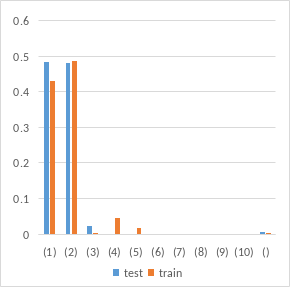
\includegraphics[width=0.31\linewidth]{figures/relative_frequencies_v10.png}
        \label{fig:relative_frequencies_v10}
    }
    \subfigure[$Lang_{13}$]{
        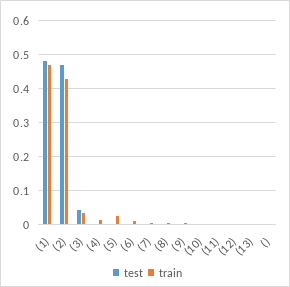
\includegraphics[width=0.31\linewidth]{figures/relative_frequencies_v13.png}
        \label{fig:relative_frequencies_v13}
    }
    \subfigure[$Lang_{100}$, (13 most frequent messages)]{
        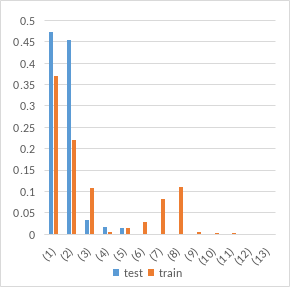
\includegraphics[width=0.31\linewidth]{figures/relative_frequencies_v100.png}
        \label{fig:relative_frequencies_v100}
    }
    \caption{Relative frequencies of messages (ordered by frequency in test dataset)}
    \label{fig:relative_frequencies_vocabularies}
\end{figure}

When looking at the emerged vocabulary \textbf{qualitatively}, a few properties can be seen.
Figure \ref{fig:relative_frequencies_vocabularies} shows an overview of the frequencies of messages in all three emerged languages for the training and the test split.
% SD: I don't understand how test and training set are used in these experiments. In language games one only has a training set and success is measured through the success in the game. It is not possible to have a test set as learning is continuous.
% DK: TODO
Since the tokens themselves are arbitrary, they are ordered by the relative frequency in the messages for the test set and indices for the tokens are added from index 1 for the most frequent token and index $|V|$ for the least frequent token.
By this the languages are easier comparable across different runs and vocabulary sizes.
% SD: I don't understand this.
% DK: TODO
Figure \ref{fig:relative_frequencies_v100} shows only the 13 most frequent message to provide a better overview.
The lesser frequent messages are never used for the test data and each only used one or two times in the train data.

The first property is that when a message is transferred, it consists of only one symbol.
% SD: Is this controlled by the sender. The sender must have some policy how it is assigning messages. Or is it just random? But what makes the sender then to generate a single message vs a longer message. If it is not controlled - how could we implement some policies for message length?
% DK: what do you mean by policy? The sender is only controled by the success of the receiver. If a longer message leads to a better success, it learns to prodcue longer messages. TODO
In some rare cases, also an empty message is communicated.
The models therefore don't learn any compositionality by combining symbols to create new meaning, but rather encode everything in separate symbols.
Secondly, in all three languages, only very few symbols occur with a high frequency, while most of the symbols are used very rarely.
More specifically, two symbols are used in 95\% of the images with $Lang_{10}$ and $Lang_{13}$, while three symbols are used with $Lang_{100}$.
Thirdly, the agents make use of fewer symbols, when presented with unseen test images compared to when communicating about images in the training split.
This is especially visible for $Lang_{100}$.
Symbols that are used for 16,5\% of the training sample are not used at all in test split.
Furthermore, the frequencies in the test split is much more focused on the two most frequent symbols, while it is more distributed around 5 symbols in the train split.
% SD: A table or a graph with these figures?
% DK: is part of the existing figure. The sum of the first two columns (QUESTION)
% SD: Differences between training and testing configuration; what happens during testing, there is no learning involved but the systems see new images but they have to use the same vocabulary?
% DK: exactly

These findings indicate that referring expressions do emerge in each of the newly emerged languages since the agents are able to communicate the correct object.
However, the agents converge towards very few different referring expressions that are made up differently than in English and likely don't rely on the high level attributes \emph{shape}, \emph{color} and \emph{size}.
% SD: Are they? We haven't tested how humans would describe these scene. I see what you mean, but they you have to explain that you count as an English expression a description containing sequences of colour, size and type and then following the Dale and Reiter's algorithm.
% DK: TODO
The similar frequencies across all three languages suggest that a greater vocabulary size $|V|$ doesn't necessarily lead to different referring expressions, but the languages still converge towards two main expressions.
% SD: All this has to do with the sender's policty how to generate messages. We should have varied this policy. I suspect no policy leads just to one message. How is the system motivated to generate more than one symbol?
% DK: TODO

\begin{figure}[ht]
    \centering
    \subfigure[$Lang_{10}$]{
        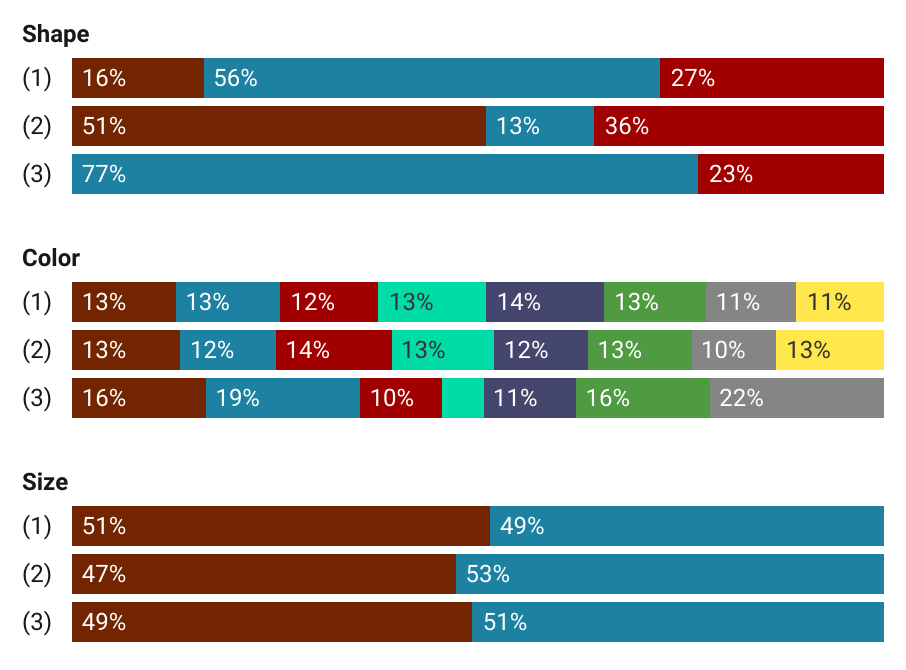
\includegraphics[width=0.31\linewidth]{figures/language_analysis_v10.png}
        \label{fig:language_analysis_v10}
    }
    \subfigure[$Lang_{13}$]{
        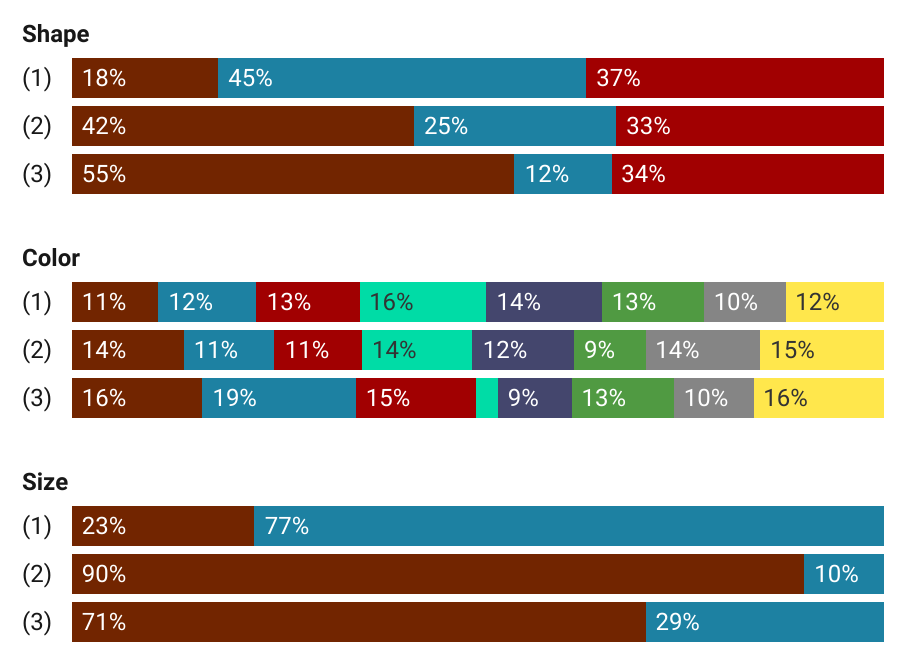
\includegraphics[width=0.31\linewidth]{figures/language_analysis_v13.png}
        \label{fig:language_analysis_v13}
    }
    \subfigure[$Lang_{100}$]{
        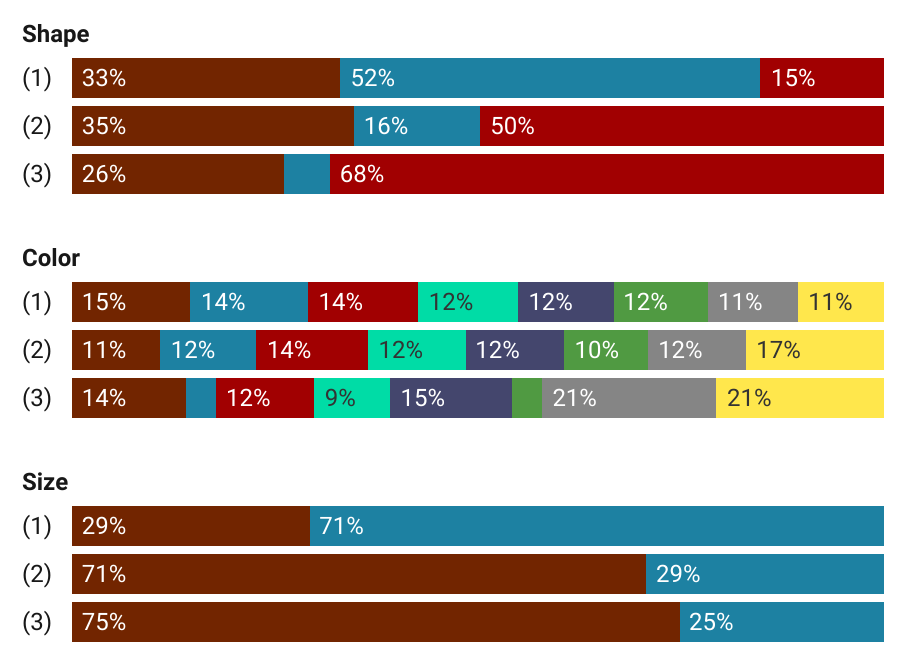
\includegraphics[width=0.31\linewidth]{figures/language_analysis_v100.png}
        \label{fig:language_analysis_v100}
    }
    \caption{Relative share of the described target object's attributes for the top three messages}

    \textbf{Shape:} brown: sphere, blue: cube, red: cylinder \\
    \textbf{Size:} brown: small, blue: large
    \label{fig:language_analysis_vocabularies}
\end{figure}

\cmtDK[inline]{differences in different languages correspond to differences in color prediction of single model caption generation}

Figure \ref{fig:language_analysis_vocabularies} shows the attributes of the target object that are described by each message.
Hereby, the relative share each value of all three attributes are displayed.
For instance the first bar in Figure \ref{fig:language_analysis_v10} shows that 16\% of the target objects that are described with symbol (1) in the language $Lang_{10}$ are spheres.
In the figures, only the three most frequently used messages are included, which make up over 95\% of all messages.

The first thing that can be seen is that different symbols convey different values of attributes.
In the language $Lang_{10}$, symbol (1) is mostly used for target objects that are cubes, while symbol (2) is mostly used for spheres.
There is not much difference for target objects that are cylinders.
The distribution for colors is almost constant across symbols (1) and (2).
Symbol (3) is more frequently used for blue, green and gray objects, while being less used for red, cyan and yellow objects.
This different distribution may also be caused by the much lower absolute usage of symbol (3).
The different sizes are encoded by all symbols in the same way.

Looking at $Lang_{13}$ the symbol usage differs.
The frequencies for the shape look similar, but (the much less used) symbol (3) encodes most of the time spheres instead of cubes.
Again, the colors look similar with small deviations for brown, green and yellow objects.
Most striking however, is the difference for the size.
Symbol (1) is used in 77\% of the cases for large objects, while symbol (2) and (3) are used in 90\% and 71\% of the messages for small objects.

Language $Lang_{100}$ uses symbols its symbols to discriminate cubes and cylinders, while the frequencies for sphere remain constant across all symbols.
The usage for the color is similar to $Lang_{13}$.
Looking at the size, as for $Lang_{13}$, symbol (1) is mostly used to encode small objects, while symbols (2) and (3) are mostly used to encode large objects.

An interesting observation is that symbols are not used for the same attributes across the languages.
In some languages, an attribute is not captured at all by the symbols, while another language heavily relies on it.
The same applies to the values of attributes, especially to the shapes.
Only two of the shapes are distinguished by the usage of symbols, while the third is not captured.
Which shape are encoded, differs from language to language.

Furthermore, these numbers confirm even more that the agents don't rely solely on the human defined attributes.
For instance $Lang_{10}$ only encodes the shape in its symbols.
This would not be enough to distinguish the target object from the distractor consistently.
Following, the agents also encode some additional underlying attributes and patterns to the three above defined attributes.
% SD: But this is slightly problematic, since we strcutured the world this way to emphasise these attributes visually. Hence, a mapping would indicate that the symbols have good semantics if they can discriminate the colours. But this could have to do with the compisitionality issue, perhaps the system was biased to use single word expressions and hence this interfered with the grounding.
% DK: TODO



